
\documentclass[12pt,onecolumn]{article}
\usepackage[brazilian]{babel}
\usepackage[utf8]{inputenc}
\usepackage{graphicx}
\usepackage{caption}
\usepackage{subcaption}
\usepackage{float}
\usepackage{hyperref}
\usepackage{blindtext}

\begin{document}

\title{Apostila de WordPress}
\author{Gustavo Teixeira da Cunha Coelho \\ Henrique Gemignani Passos Lima}
\maketitle

\section{Sobre o WordPress}
	TODO: O wordpress é dahora.

\section{Instalando}
	O \href{http://codex.wordpress.org/Installing_WordPress}{guia oficial} do 
	WordPress cobre todos os casos comuns, então nada melhor que utilizar a documentação oficial.
	
	TODO: tecer alguns comentários sobre a instalação, mesmo assim. \blindtext

\section{Postando}

	\subsection{Autorização}
		É importante notar que o WordPress possui um controle de acesso, logo 
		somente pessoas autorizadas podem criar novos posts.
		
		Para tal, precisamos então realizar o login.
		\begin{figure}[H]
			\begin{subfigure}{.4\textwidth}
				\centering
				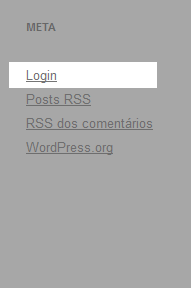
\includegraphics{login1.png}
				\caption{Link para a página de login}
			\end{subfigure}
			\begin{subfigure}{.4\textwidth}
				\centering
				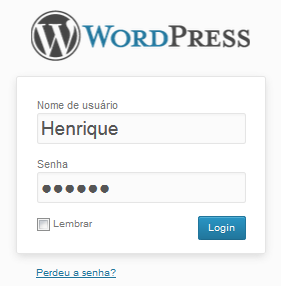
\includegraphics{login2.png}
				\caption{Digitando usuário e senha}
			\end{subfigure}
			\caption{Processo de login}
		\end{figure}
	
	\subsection{Criando um post}
		TODO: é simples que só imagens bastam
		\begin{figure}[H]
			\centering
			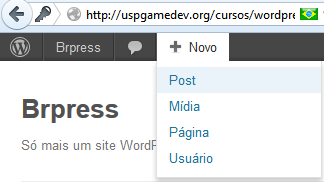
\includegraphics{post1.png}
			\caption{Usando a barra do WordPress}
		\end{figure}
		\begin{figure}[H]
			\centering
			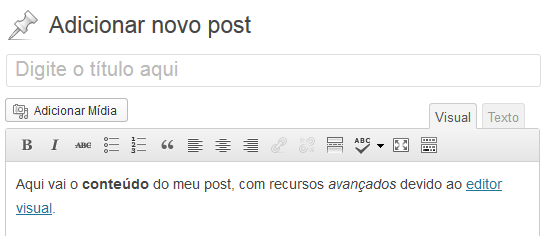
\includegraphics{post2.png}
			\caption{Usando o editor visual}
		\end{figure}
		\begin{figure}[H]
			\centering
			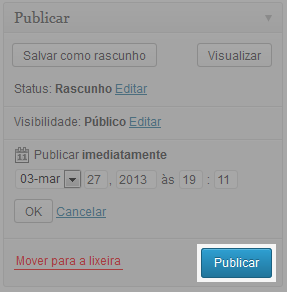
\includegraphics{post3.png}
			\caption{Publicando}
		\end{figure}

	\subsection{Páginas}
		Um tipo especial de post no Wordpress são as Páginas.
		Essas páginas são tratadas de maneira especial pelo seu tema, como por
		exemplo listando todas na página inicial.
		\begin{figure}[H]
			\centering
			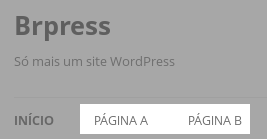
\includegraphics{page1.png}
			\caption{Lista de páginas do tema padrão}
		\end{figure}
		
\section{Conteúdo Elaborado}
	Não é apenas de texto que o blog vai ficar bom.
	\subsection{Imagens}
		Adicionar imagens no seu post é simples, basta clica em Adicionar Mídia.
		\begin{figure}[H]
			\centering
			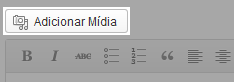
\includegraphics{midia1.png}
			\caption{Botão 'Adicionar Mídia'.}
		\end{figure}
		Feito isso, você pode ou enviar novas imagens para o site ou utilizar 
		aquelas que já estão disponíveis na aba Biblioteca de Mídia.
	\subsection{Vídeos}
		A forma mais fácil é enviar o vídeo para algum dos sites que o 
		\href{http://codex.wordpress.org/Embeds}{WordPress tem suporte} e 
		então colocar o link no post. O resto acontece sozinho.
		
\end{document}
